\chapter{System Design and Diagrams}

\section{Overview of System Design}

System design is the foundational phase within the Software Development Life Cycle (SDLC) where user requirements, business logic, and operational constraints specified in the Software Requirement Specification (SRS) are transformed into a concrete technical blueprint. In accordance with established software engineering paradigms, system design encompasses both architectural (high-level) design and detailed (low-level) design.

High-level design focuses on the macro-level decomposition of the system into modular subsystems, structural packages, external interfaces, and deployment topologies. Low-level design details the internal logic, algorithms, state transitions, message sequences, and relational structures that govern the runtime behavior of individual system components.

For the \textbf{Bank Loan Management System}, design modeling is approached through two complementary software engineering viewpoints:

\begin{enumerate}
  \item \textbf{Function-Oriented Modeling (Structured Analysis and Design):} Utilizes Data Flow Diagrams (DFDs) to trace the functional transformation of data across system boundaries, and Structure Charts to document top-down modular decomposition, functional cohesion, and inter-module coupling.
  \item \textbf{Object-Oriented Modeling (Unified Modeling Language - UML):} Employs standard structural and behavioral diagrams (Use Case, Class, Object, State-Chart, Activity, Sequence, Collaboration, Component, and Deployment diagrams) to capture encapsulation, inheritance hierarchies, runtime object lifecycles, and asynchronous inter-component interactions.
\end{enumerate}

Every diagram included in this chapter models the same proposed Bank Loan Management System, ensuring strict semantic, behavioral, and structural consistency across the entire documentation.

\section{Problem Flowchart (Beyond Syllabus Experiment 1)}

A flowchart is a standard algorithmic tool used to depict the sequential flow of execution, decision nodes, input/output operations, and control branches governing a business process. In the context of the Bank Loan Management System, the problem flowchart models the complete lifecycle of a loan transaction from initial customer onboarding to final loan closure upon complete repayment.

The workflow begins with customer authentication. Unregistered users are directed to the registration module where mandatory identity parameters (PAN, Aadhaar, contact details) are captured and validated. Upon successful authentication, the customer navigates to the loan catalog, selects an appropriate credit product (Home Loan, Personal Loan, Education Loan, Vehicle Loan), inputs financial metrics (annual income, requested amount, repayment tenure), and uploads mandatory documentary evidence.

The system subsequently executes automated format and integrity checks on uploaded documents. If the documentation is defective, the customer is prompted for re-submission. Valid applications undergo eligibility screening against pre-configured risk assessment algorithms (debt-to-income ratio, credit score, disposable income). If the applicant fails eligibility thresholds, an automated rejection notice is generated. Qualifying applications are forwarded to the Bank Employee dashboard for credit appraisal. The employee exercises sanctioning authority, approving or rejecting the proposal.

Upon approval, the system generates a definitive loan account, computes the Equated Monthly Installment (EMI) amortization schedule using compound interest algorithms, and initiates fund disbursement. The customer subsequently services the loan through periodic monthly payments. Each repayment is logged against the loan balance, dynamically recalculating outstanding principal and accrued interest. When the cumulative repayments satisfy the total debt obligation, the system updates the account status to 'Closed', generates a formal No Objection Certificate (NOC), and terminates the active loan lifecycle.

\begin{figure}[htbp]
\centering
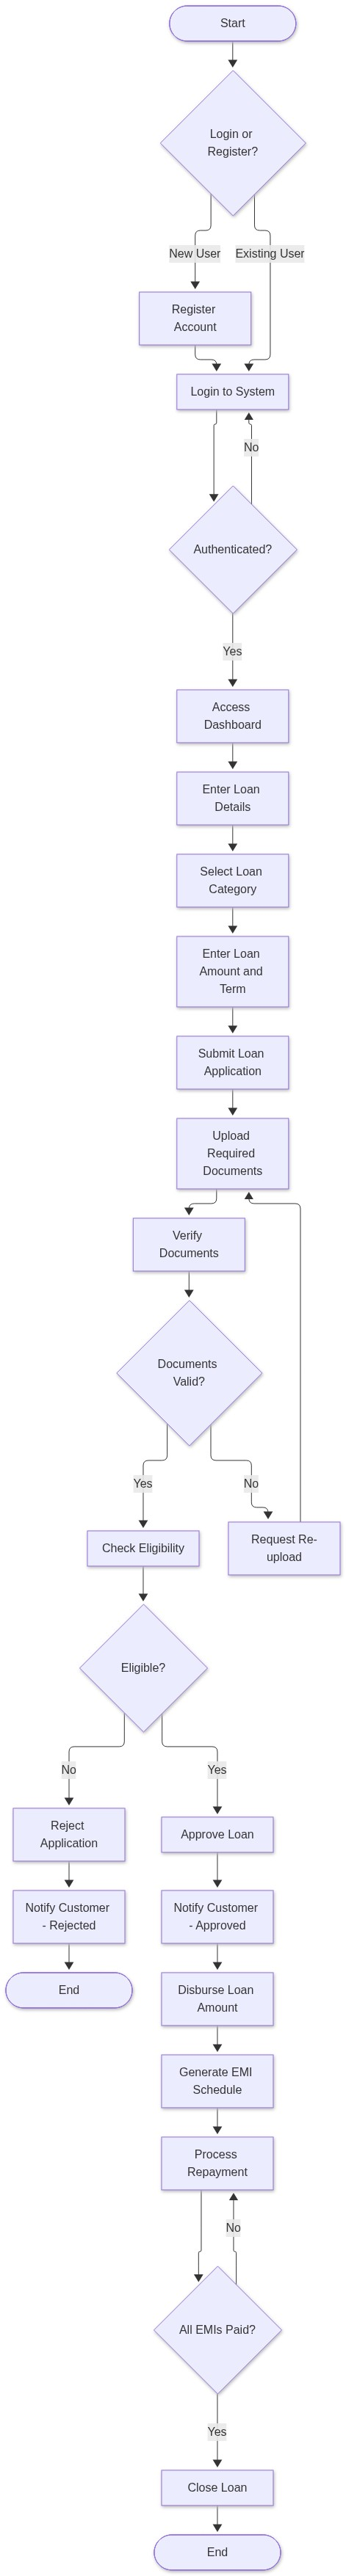
\includegraphics[width=0.85\textwidth]{figures/flowchart.png}
\caption{Figure 3.1: Problem Flowchart of the Bank Loan Management System}
\label{fig:flowchart}
\end{figure}

\textit{Figure 3.1: Problem Flowchart of the Bank Loan Management System}

\section{Data Flow Diagrams (DFD) (Experiment 3)}

A Data Flow Diagram (DFD) is a graphical modeling technique that represents the flow of data through an information system, illustrating the functional processes that transform incoming data streams into outgoing results, the external entities that act as data sources or sinks, and the persistent data repositories that maintain system state.

\subsection{Context-Level DFD (Level 0)}

The Context-Level DFD represents the entire Bank Loan Management System as a single centralized software process (Process 0.0), delimiting the operational boundaries of the application and detailing its external data exchanges with interacting stakeholders.

The system interfaces with three primary external entities:

\begin{enumerate}
  \item \textbf{Customer:} Supplies customer registration credentials, completed loan applications, KYC/income documents, loan tracking queries, and EMI repayment payments. Receives account status alerts, eligibility estimates, sanction letters, EMI amortization schedules, and digital payment receipts.
  \item \textbf{Bank Employee (Loan Officer / Credit Analyst):} Retrieves pending loan applications, inspection queues, and customer financial profiles. Submits document verification evaluations, credit underwriting decisions, and approval/rejection authorizations.
  \item \textbf{Administrator:} Submits user authorization policies, loan category configurations, interest rate revisions, and audit inquiries. Receives comprehensive business intelligence reports, portfolio performance analytics, and system audit logs.
\end{enumerate}

\begin{figure}[htbp]
\centering
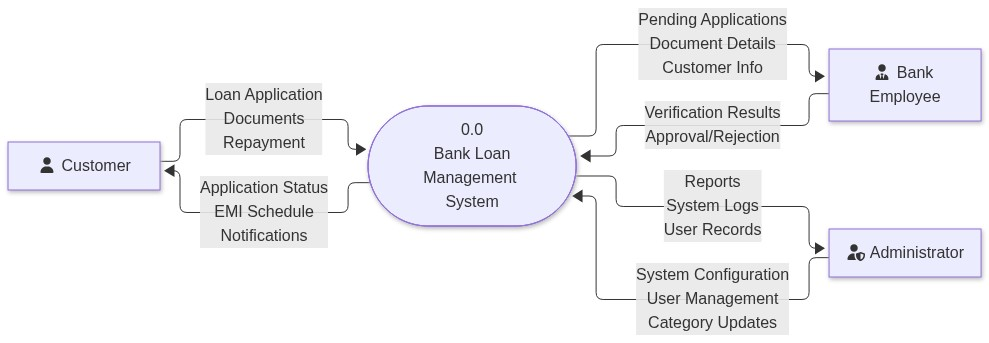
\includegraphics[width=0.85\textwidth]{figures/dfd_level_0.png}
\caption{Figure 3.2: Context-Level Data Flow Diagram (Level 0)}
\label{fig:dfd_level_0}
\end{figure}

\textit{Figure 3.2: Context-Level Data Flow Diagram (Level 0)}

\subsection{First-Level DFD (Level 1)}

The Level 1 DFD decomposes the monolithic Context DFD into six core business processes, explicitly delineating data interactions between individual processes and the underlying persistent data stores:

\begin{itemize}
  \item \textbf{Process 1.0 (User Registration and Authentication):} Validates new user credentials, hashes passwords, generates authentication tokens, and writes user records to \textbf{D1: User Database}.
  \item \textbf{Process 2.0 (Loan Application Processing):} Accepts requested loan parameters, performs preliminary input validation, generates a unique Application ID, and persists application records in \textbf{D2: Loan Application Database}.
  \item \textbf{Process 3.0 (Document Verification and Eligibility Assessment):} Accepts digital document uploads, writes metadata to \textbf{D3: Document Database}, triggers verification workflows for Bank Employees, and executes algorithmic credit score calculations.
  \item \textbf{Process 4.0 (Loan Approval and Rejection Management):} Captures underwriting decisions made by Bank Employees, updates application state, generates sanction letters, and instantiates approved loans in \textbf{D4: Loan Records Database}.
  \item \textbf{Process 5.0 (EMI and Repayment Management):} Calculates amortization schedules, tracks incoming EMI remittances, updates outstanding principal, logs transactions in \textbf{D5: Repayment Database}, and issues account closure statements.
  \item \textbf{Process 6.0 (System Administration and Reporting):} Administers employee roles, manages loan product categories, monitors regulatory compliance, and aggregates multi-table records to generate analytical management reports.
\end{itemize}

\begin{figure}[htbp]
\centering
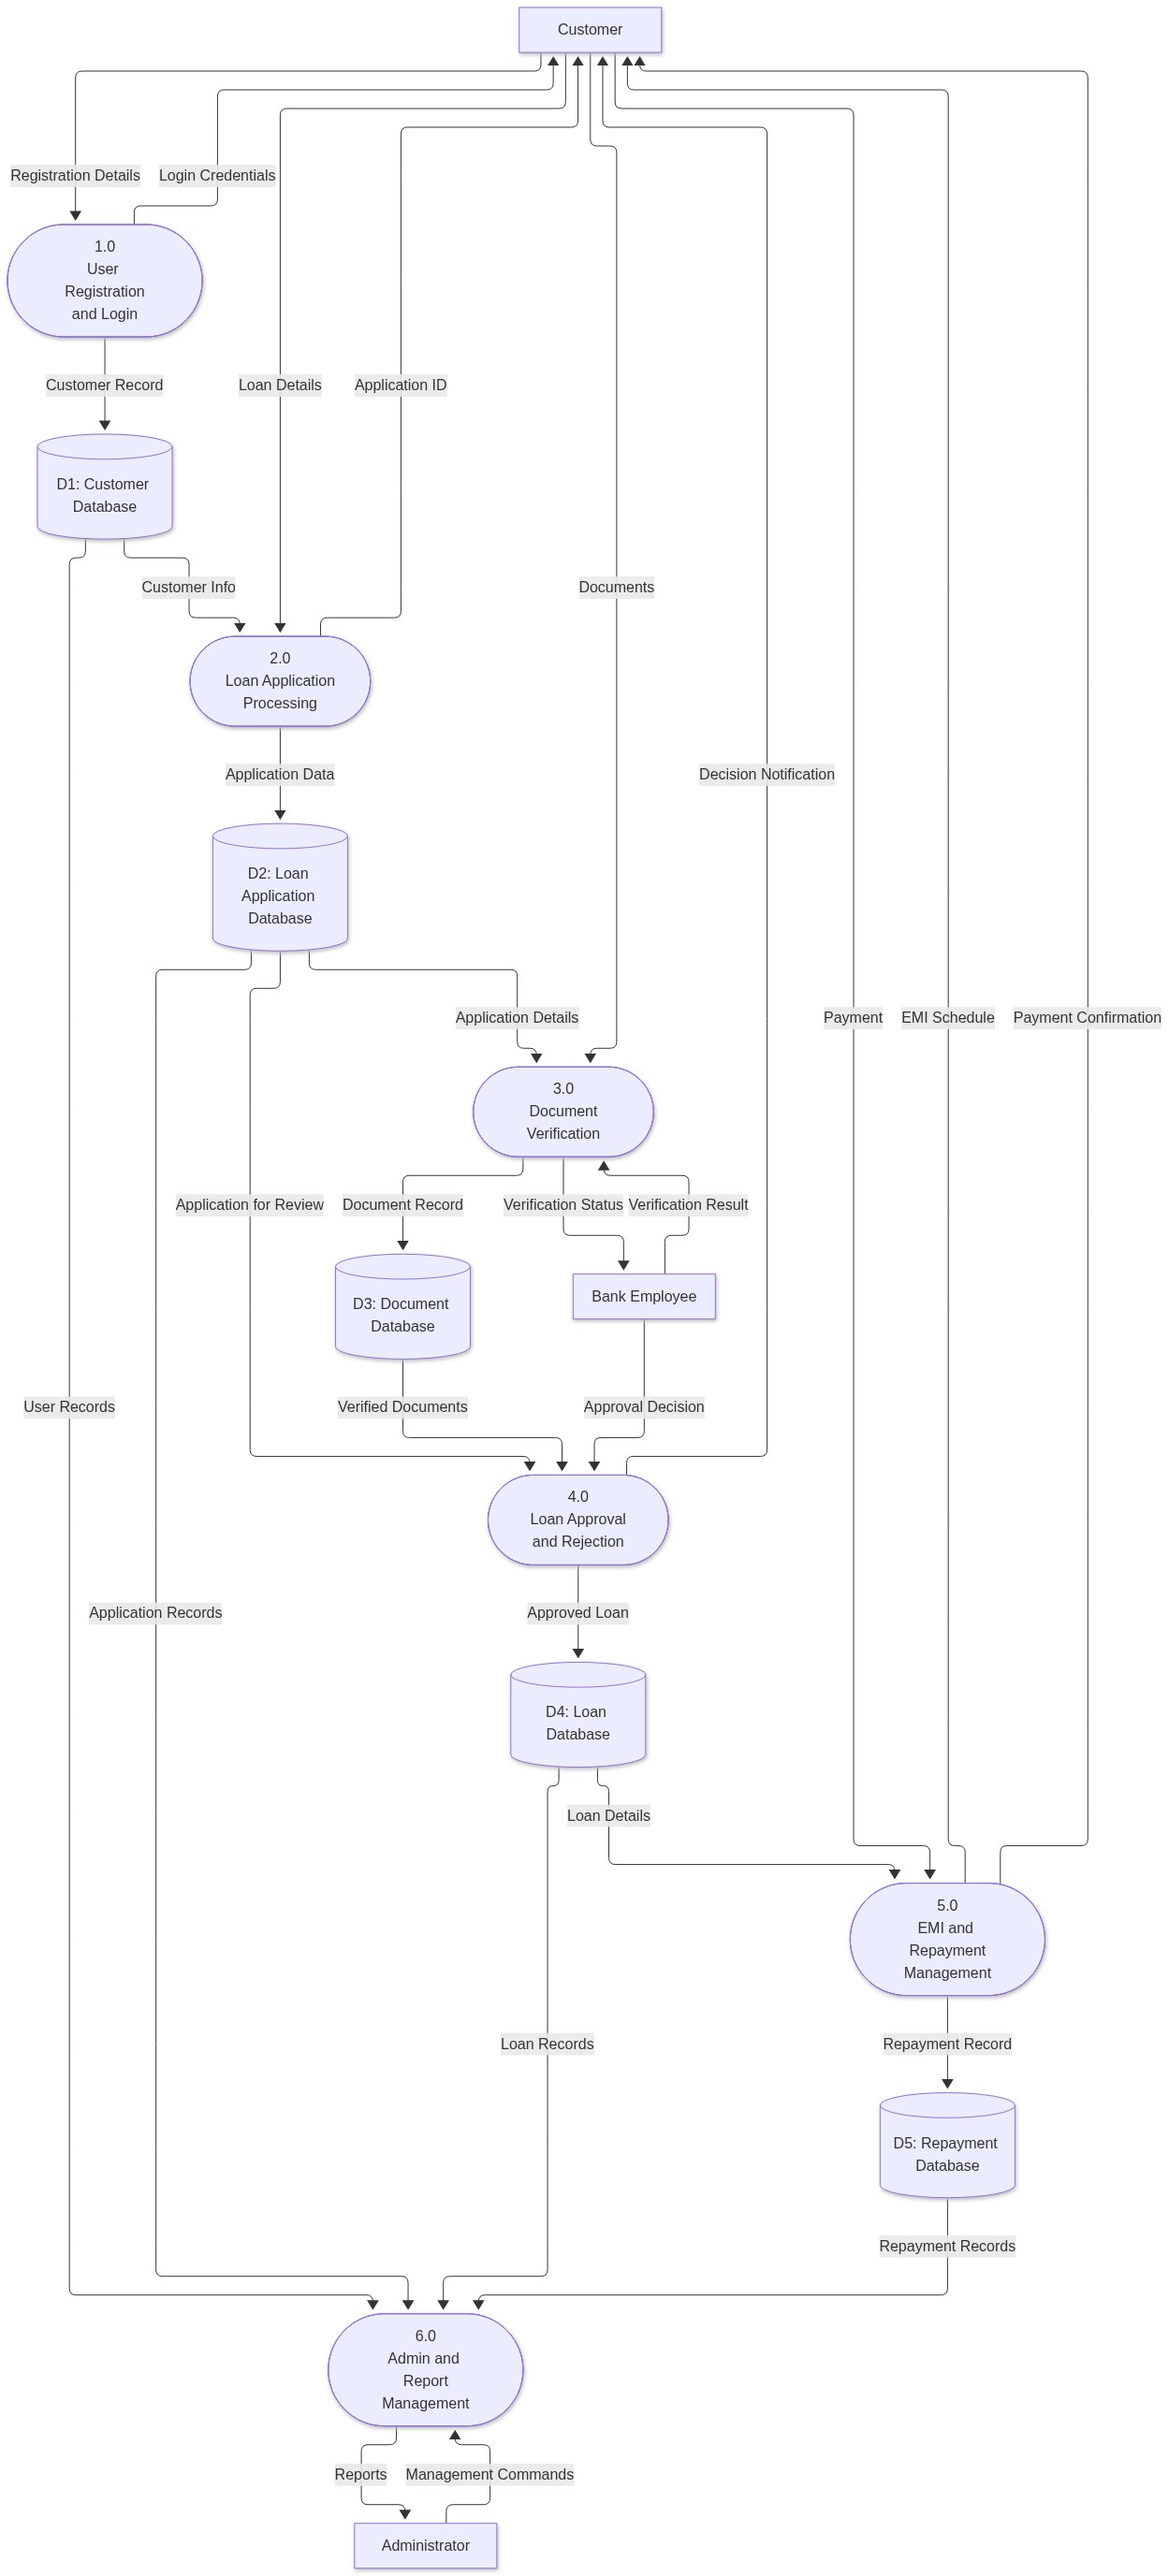
\includegraphics[width=0.85\textwidth]{figures/dfd_level_1.png}
\caption{Figure 3.3: First-Level Data Flow Diagram (Level 1)}
\label{fig:dfd_level_1}
\end{figure}

\textit{Figure 3.3: First-Level Data Flow Diagram (Level 1)}

\subsection{Second-Level DFD (Level 2 - Process 2.0: Loan Application Processing)}

To provide deeper insight into critical business workflows, Process 2.0 (Loan Application Processing) is further decomposed into its constituent sub-processes:

\begin{itemize}
  \item \textbf{Process 2.1 (Select Loan Category):} Retrieves active loan schemes, interest rates, and loan term constraints from the database and presents valid options to the user.
  \item \textbf{Process 2.2 (Capture Applicant Details):} Validates and captures applicant demographic, employment, salary, and liability data.
  \item \textbf{Process 2.3 (Evaluate Preliminary Eligibility):} Evaluates applicant criteria against product eligibility rules, returning immediate indicative eligibility feedback.
  \item \textbf{Process 2.4 (Assemble Application Package):} Binds applicant data, loan parameters, and preliminary scores into a consolidated application payload.
  \item \textbf{Process 2.5 (Persist Application \& Generate Tracking ID):} Writes the record to \textbf{D2: Loan Application Database} and returns a unique tracking reference to the applicant.
\end{itemize}

\begin{figure}[htbp]
\centering
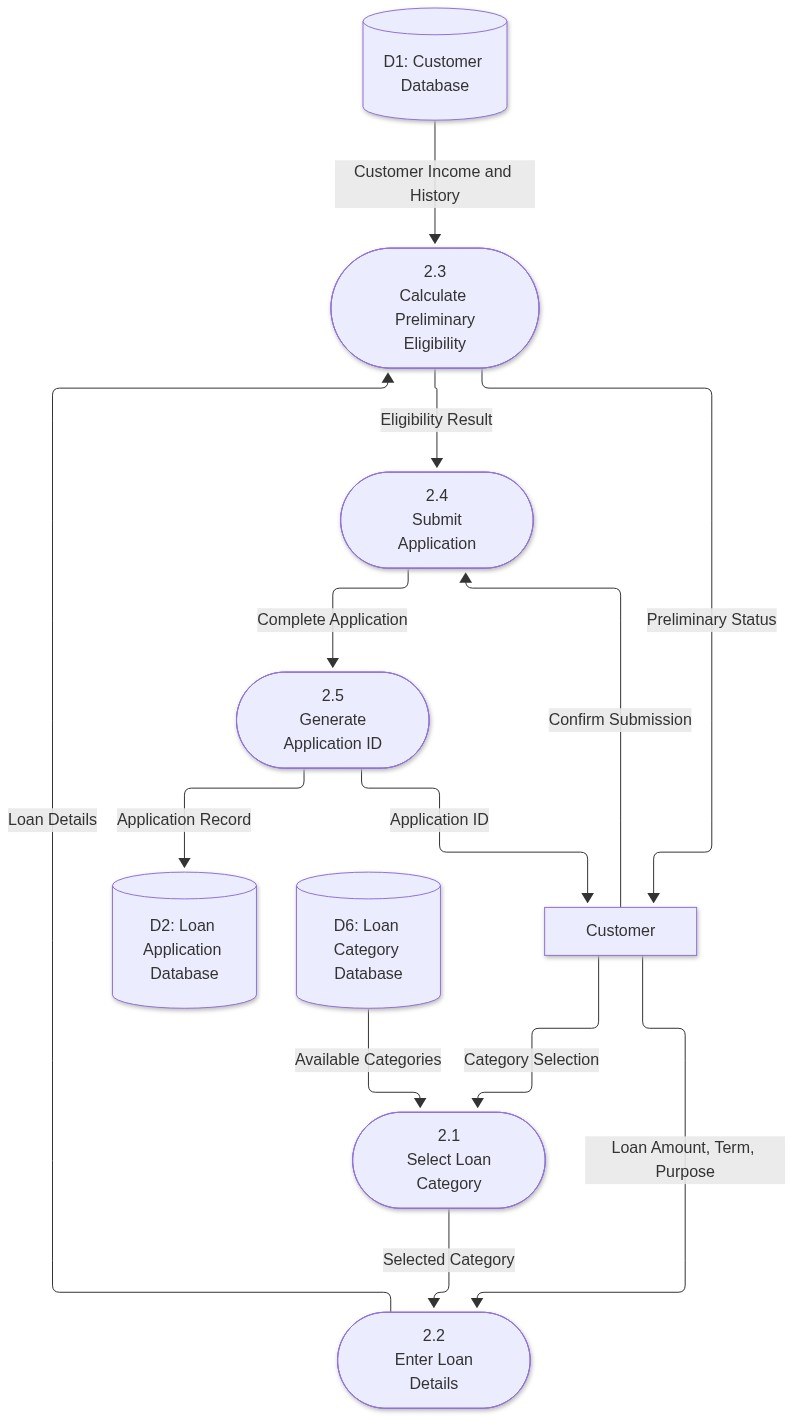
\includegraphics[width=0.85\textwidth]{figures/dfd_level_2.png}
\caption{Figure 3.4: Second-Level Data Flow Diagram (Level 2 - Loan Application Processing)}
\label{fig:dfd_level_2}
\end{figure}

\textit{Figure 3.4: Second-Level Data Flow Diagram (Level 2 - Loan Application Processing)}

\section{Structure Chart (Experiment 3)}

A Structure Chart models the functional architecture of a software system in a top-down hierarchical manner. It portrays the partitioning of the program into discrete modules, illustrating invocation relationships, data coupling (parameters passed between modules), and control flags (decision indicators returned by submodules).

The top-level executive module \textbf{0.0 Bank Loan Management System} orchestrates six principal functional subsystems:

\begin{enumerate}
  \item \textbf{Module 1.0 User Management:} Subdivided into \textit{1.1 Register Customer}, \textit{1.2 Authenticate Credentials}, and \textit{1.3 Manage Profile Details}.
  \item \textbf{Module 2.0 Loan Application Management:} Subdivided into \textit{2.1 Select Loan Scheme}, \textit{2.2 Input Financial Details}, and \textit{2.3 Upload Application Documents}.
  \item \textbf{Module 3.0 Verification Management:} Subdivided into \textit{3.1 Inspect KYC Documents}, \textit{3.2 Compute Credit Score}, and \textit{3.3 Assess Repayment Capacity}.
  \item \textbf{Module 4.0 Approval Management:} Subdivided into \textit{4.1 Review Application Queue}, \textit{4.2 Authorize Loan Sanction}, and \textit{4.3 Reject Ineligible Proposal}.
  \item \textbf{Module 5.0 Repayment Management:} Subdivided into \textit{5.1 Compute EMI Schedule}, \textit{5.2 Record Installment Remittance}, and \textit{5.3 Process Loan Closure}.
  \item \textbf{Module 6.0 Administration and Reporting:} Subdivided into \textit{6.1 Manage User Accounts}, \textit{6.2 Configure Loan Categories}, and \textit{6.3 Generate Audit Reports}.
\end{enumerate}

Each module exhibits high functional cohesion (performing a single, well-defined operational task) and low inter-module coupling (interacting primarily through clean parameter passing), ensuring optimal maintainability, extensibility, and testability.

\begin{figure}[htbp]
\centering
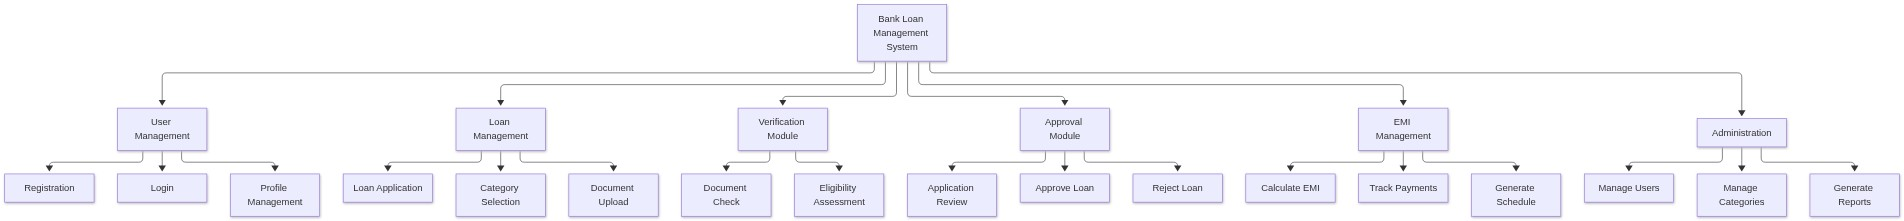
\includegraphics[width=0.85\textwidth]{figures/structure_chart.png}
\caption{Figure 3.5: System Structure Chart}
\label{fig:structure_chart}
\end{figure}

\textit{Figure 3.5: System Structure Chart}

\section{Entity-Relationship Diagram (ERD) (Experiment 4 \& Beyond Syllabus Exp 2)}

The Entity-Relationship (ER) Diagram provides the conceptual schema for the persistent data store of the Bank Loan Management System. It models the core real-world business entities, their descriptive attributes, primary keys, foreign key constraints, and relational cardinalities.

The conceptual schema comprises six fundamental entities:

\begin{enumerate}
  \item \textbf{CUSTOMER:} Captures borrower demographic and financial profiles.
\end{enumerate}

\begin{itemize}
  \item Primary Key: \texttt{Customer\_ID}
  \item Attributes: \texttt{Name}, \texttt{DOB}, \texttt{Address}, \texttt{Phone\_Number}, \texttt{Email}, \texttt{Income}, \texttt{Password\_Hash}, \texttt{Registration\_Date}
\end{itemize}

\begin{enumerate}
  \item \textbf{LOAN\_APPLICATION:} Represents formal requests for credit submitted by customers.
\end{enumerate}

\begin{itemize}
  \item Primary Key: \texttt{Application\_ID}
  \item Foreign Keys: \texttt{Customer\_ID} (references CUSTOMER), \texttt{Employee\_ID} (references BANK\_EMPLOYEE)
  \item Attributes: \texttt{Loan\_Type}, \texttt{Loan\_Amount}, \texttt{Tenure\_Months}, \texttt{Application\_Date}, \texttt{Application\_Status}, \texttt{Remarks}
\end{itemize}

\begin{enumerate}
  \item \textbf{BANK\_EMPLOYEE:} Maintains internal bank staff credentials and supervisory roles.
\end{enumerate}

\begin{itemize}
  \item Primary Key: \texttt{Employee\_ID}
  \item Attributes: \texttt{Employee\_Name}, \texttt{Designation}, \texttt{Email}, \texttt{Phone\_Number}, \texttt{Department}, \texttt{Role}
\end{itemize}

\begin{enumerate}
  \item \textbf{DOCUMENT:} Stores verification records and binary attachment pointers for submitted applications.
\end{enumerate}

\begin{itemize}
  \item Primary Key: \texttt{Document\_ID}
  \item Foreign Key: \texttt{Application\_ID} (references LOAN\_APPLICATION)
  \item Attributes: \texttt{Document\_Type}, \texttt{File\_Path}, \texttt{Upload\_Date}, \texttt{Verification\_Status}, \texttt{Verified\_Date}
\end{itemize}

\begin{enumerate}
  \item \textbf{LOAN:} Represents fully approved and disbursed credit accounts.
\end{enumerate}

\begin{itemize}
  \item Primary Key: \texttt{Loan\_ID}
  \item Foreign Key: \texttt{Application\_ID} (references LOAN\_APPLICATION)
  \item Attributes: \texttt{Loan\_Amount}, \texttt{Interest\_Rate}, \texttt{Loan\_Term}, \texttt{Approval\_Date}, \texttt{Disbursement\_Date}, \texttt{Loan\_Status}, \texttt{Outstanding\_Balance}
\end{itemize}

\begin{enumerate}
  \item \textbf{REPAYMENT:} Tracks periodic installment payments against active loan accounts.
\end{enumerate}

\begin{itemize}
  \item Primary Key: \texttt{Repayment\_ID}
  \item Foreign Key: \texttt{Loan\_ID} (references LOAN)
  \item Attributes: \texttt{EMI\_Amount}, \texttt{Principal\_Paid}, \texttt{Interest\_Paid}, \texttt{Due\_Date}, \texttt{Payment\_Date}, \texttt{Payment\_Status}, \texttt{Late\_Penalty}
\end{itemize}

\subsection{Cardinality and Participation Rules}

\begin{itemize}
  \item \textbf{CUSTOMER to LOAN\_APPLICATION (1:M):} One customer can submit multiple loan applications.
  \item \textbf{LOAN\_APPLICATION to LOAN (1:0..1):} An application may generate at most one approved loan.
  \item \textbf{LOAN\_APPLICATION to DOCUMENT (1:M):} One application contains multiple supporting documents.
  \item \textbf{BANK\_EMPLOYEE to LOAN\_APPLICATION (1:M):} One employee verifies multiple applications.
  \item \textbf{LOAN to REPAYMENT (1:M):} One loan has multiple monthly repayment records.
\end{itemize}

\begin{figure}[htbp]
\centering
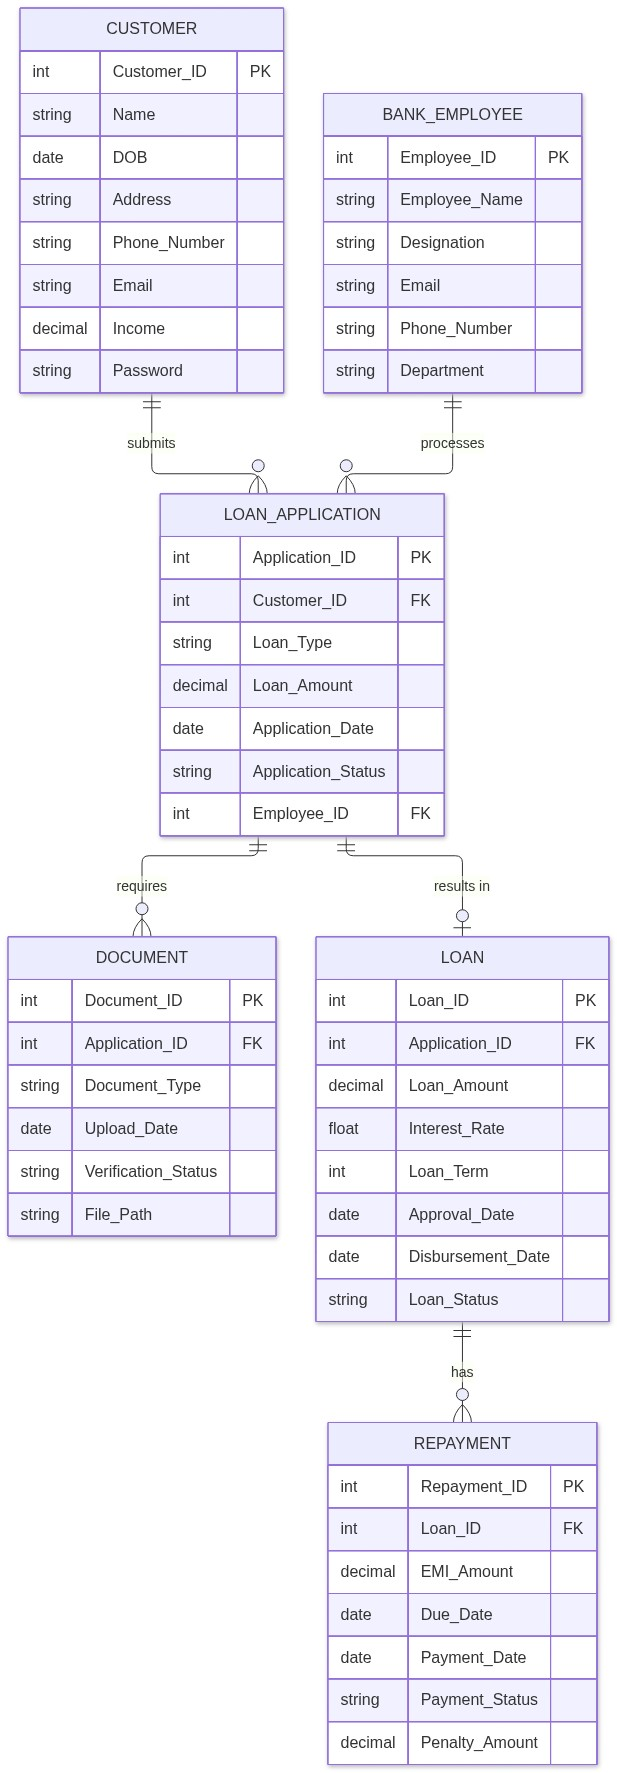
\includegraphics[width=0.85\textwidth]{figures/er_diagram.png}
\caption{Figure 3.6: Entity-Relationship Diagram (ERD)}
\label{fig:er_diagram}
\end{figure}

\textit{Figure 3.6: Entity-Relationship Diagram (ERD)}

\section{Use Case Diagram (Experiment 5)}

The UML Use Case Diagram captures the behavioral view of the system from the perspective of external actors. It delineates the functional boundary of the software application, mapping external roles to the specific use cases (services or operations) they initiate or interact with.

\subsection{Actors}

\begin{itemize}
  \item \textbf{Customer:} Primary external user seeking credit facilities, monitoring progress, and servicing repayments.
  \item \textbf{Bank Employee (Credit Officer):} Internal staff member responsible for KYC verification, applicant financial appraisal, and sanction decisions.
  \item \textbf{Administrator:} Technical supervisor responsible for platform maintenance, security configurations, product definitions, and compliance auditing.
\end{itemize}

\subsection{Key Use Cases and Stereotypes}

\begin{itemize}
  \item \texttt{\guillemotleft{}include\guillemotright{}} Relationships:
  \item \textit{Submit Loan Application} \textbf{\guillemotleft{}include\guillemotright{}} \textit{Authenticate Customer}
  \item \textit{Submit Loan Application} \textbf{\guillemotleft{}include\guillemotright{}} \textit{Select Loan Category}
  \item \textit{Assess Loan Eligibility} \textbf{\guillemotleft{}include\guillemotright{}} \textit{Verify Customer Documents}
  \item \texttt{\guillemotleft{}extend\guillemotright{}} Relationships:
  \item \textit{Track Application Status} \textbf{\guillemotleft{}extend\guillemotright{}} \textit{View Rejection Reason}
  \item \textit{Make Loan Repayment} \textbf{\guillemotleft{}extend\guillemotright{}} \textit{Apply Late Penalty}
\end{itemize}

\begin{figure}[htbp]
\centering
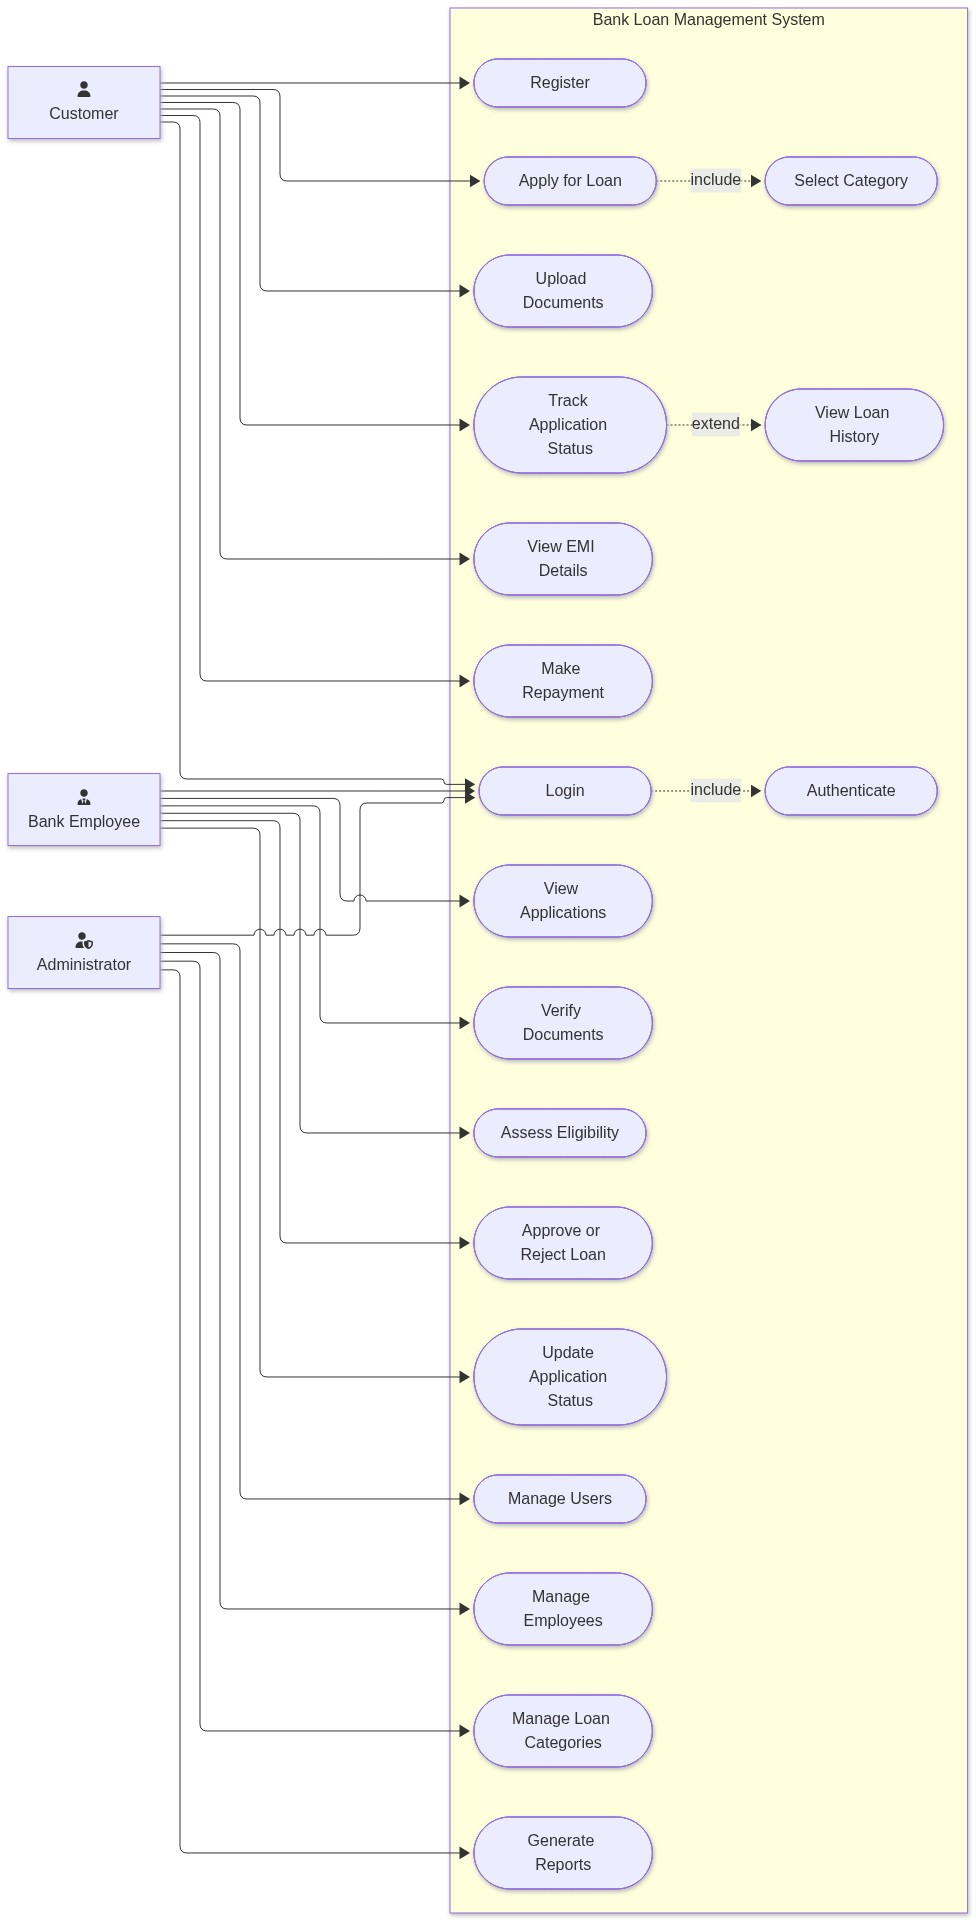
\includegraphics[width=0.85\textwidth]{figures/use_case_diagram.png}
\caption{Figure 3.7: Use Case Diagram}
\label{fig:use_case_diagram}
\end{figure}

\textit{Figure 3.7: Use Case Diagram}

\section{Class Diagram (Experiment 6)}

The UML Class Diagram models the static structural foundation of the Bank Loan Management System. It details system classes, encapsulated attributes (with visibility modifiers and data types), behavioral member methods, inheritance hierarchies, and associative relationships.

\subsection{Class Hierarchy and Encapsulation}

\begin{itemize}
  \item \textbf{User (Abstract Base Class):} Encapsulates universal authentication properties (\texttt{userId: String}, \texttt{username: String}, \texttt{passwordHash: String}, \texttt{email: String}, \texttt{role: String}) and shared methods (\texttt{login(): Boolean}, \texttt{logout(): Void}, \texttt{updateProfile(): Boolean}).
  \item \textbf{Customer (Subclass of User):} Inherits from \texttt{User}, adding domain-specific borrower attributes (\texttt{customerId: String}, \texttt{name: String}, \texttt{dob: Date}, \texttt{address: String}, \texttt{phone: String}, \texttt{monthlyIncome: Double}) and member operations (\texttt{register(): Boolean}, \texttt{applyForLoan(): LoanApplication}, \texttt{uploadDocument(): Document}, \texttt{trackStatus(): String}, \texttt{makeRepayment(): Boolean}).
  \item \textbf{BankEmployee (Subclass of User):} Extends \texttt{User} with credit processing attributes (\texttt{employeeId: String}, \texttt{designation: String}, \texttt{department: String}) and administrative operations (\texttt{viewApplications(): List}, \texttt{verifyDocuments(): Boolean}, \texttt{assessEligibility(): Double}, \texttt{approveRejectLoan(): Void}).
  \item \textbf{Administrator (Subclass of User):} Extends \texttt{User} with platform governance capabilities (\texttt{adminId: String}, \texttt{manageUsers(): Void}, \texttt{configureLoanCategories(): Void}, \texttt{generateReports(): Report}).
  \item \textbf{LoanApplication:} Represents loan proposals (\texttt{applicationId: String}, \texttt{loanType: String}, \texttt{amount: Double}, \texttt{tenure: Int}, \texttt{status: String}, \texttt{submissionDate: Date}).
  \item \textbf{Document:} Encapsulates uploaded evidence (\texttt{documentId: String}, \texttt{docType: String}, \texttt{filePath: String}, \texttt{verificationStatus: String}).
  \item \textbf{Loan:} Represents funded accounts (\texttt{loanId: String}, \texttt{sanctionedAmount: Double}, \texttt{interestRate: Double}, \texttt{tenureMonths: Int}, \texttt{outstandingBalance: Double}, \texttt{calculateEMI(): Double}, \texttt{disburseFunds(): Void}).
  \item \textbf{Repayment:} Models installment transactions (\texttt{repaymentId: String}, \texttt{emiAmount: Double}, \texttt{dueDate: Date}, \texttt{paymentDate: Date}, \texttt{status: String}, \texttt{processPayment(): Boolean}).
  \item \textbf{LoanCategory:} Catalogs credit products (\texttt{categoryId: String}, \texttt{categoryName: String}, \texttt{minAmount: Double}, \texttt{maxAmount: Double}, \texttt{interestRate: Double}, \texttt{maxTenure: Int}).
\end{itemize}

\begin{figure}[htbp]
\centering
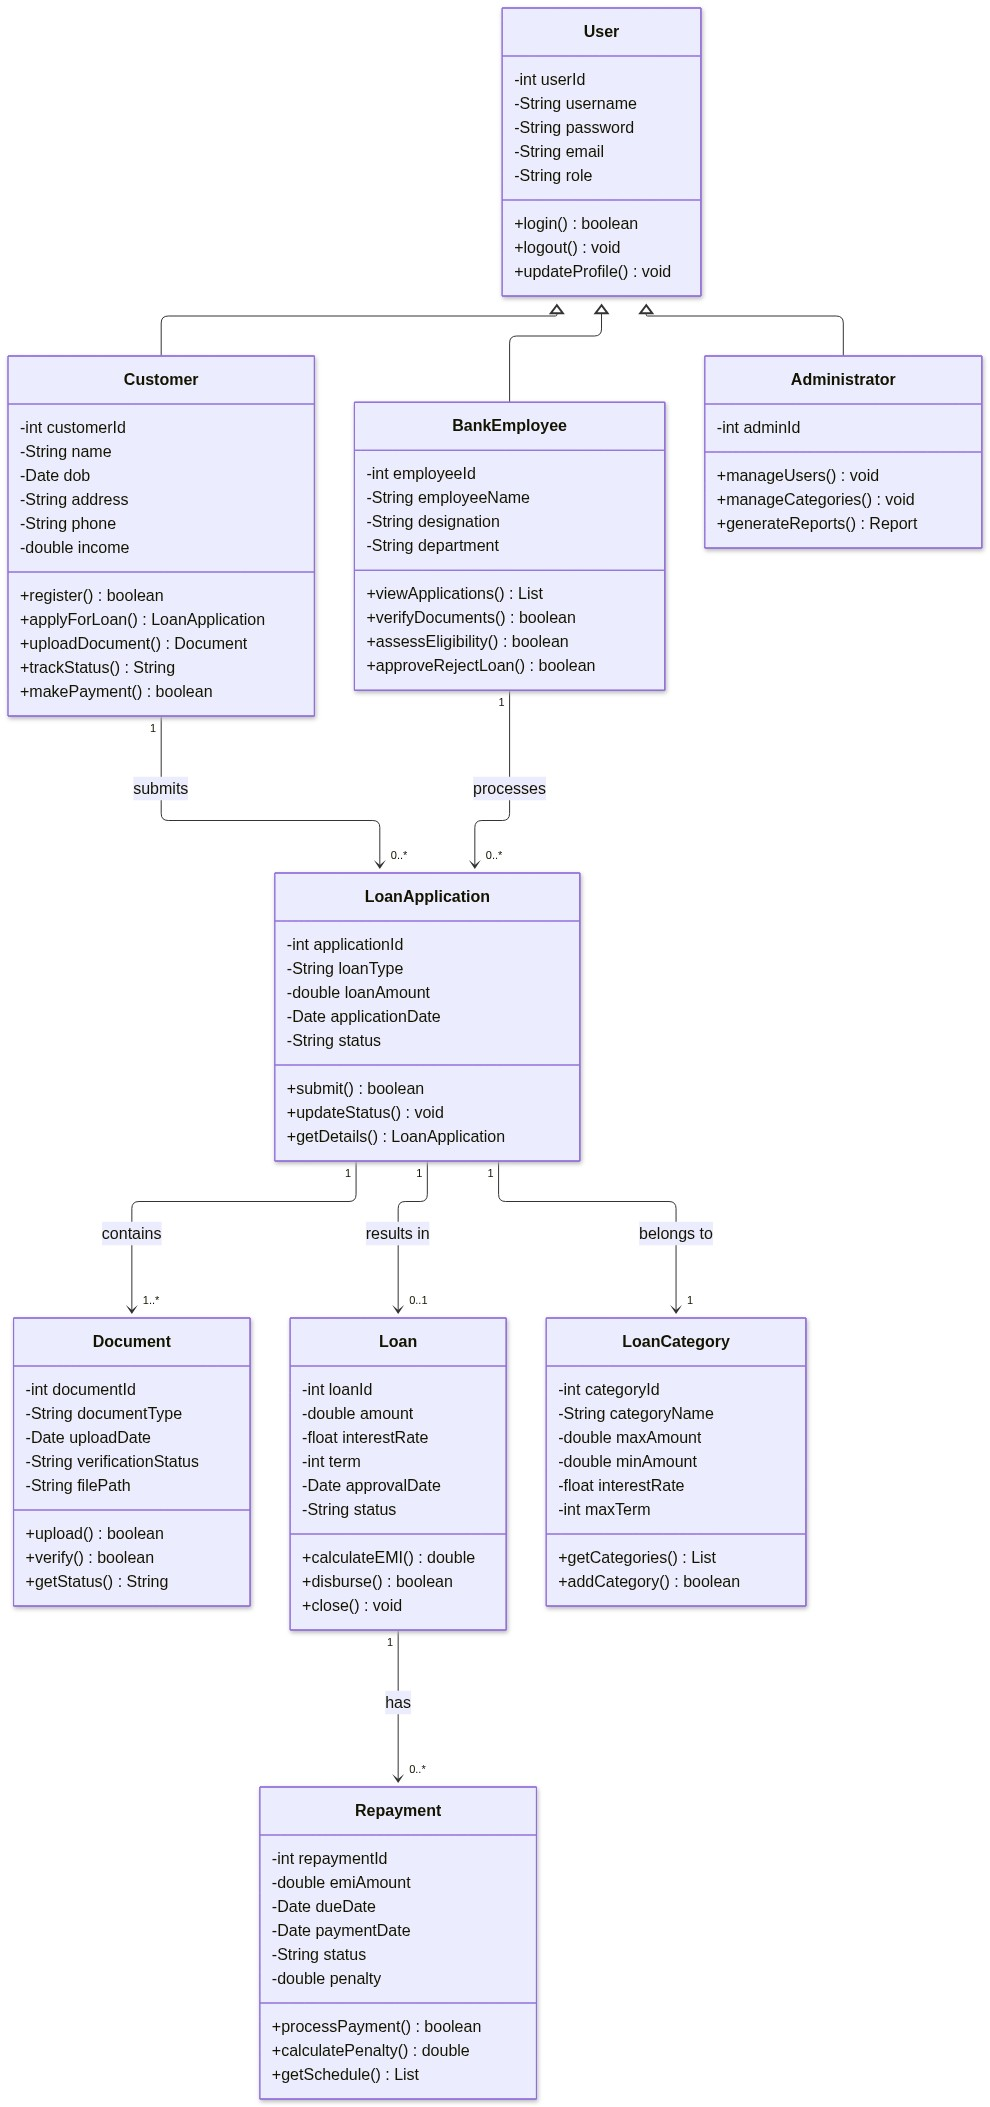
\includegraphics[width=0.85\textwidth]{figures/class_diagram.png}
\caption{Figure 3.8: Class Diagram}
\label{fig:class_diagram}
\end{figure}

\textit{Figure 3.8: Class Diagram}

\section{Object Diagram (Experiment 6)}

An Object Diagram represents a concrete runtime snapshot of class instances and their inter-object associations at a specific moment in system execution. It validates the correctness of the static class structure by demonstrating how instantiated objects hold concrete attribute values and reference each other.

The depicted instance scenario captures customer \texttt{cust1:Customer} (Rahul Sharma, Income: INR 75,000/mo) who has applied for a home loan (\texttt{app1:LoanApplication}, Amount: INR 2,500,000, 240 months tenure). The application has associated identity documentation (\texttt{doc1:Document}, Type: "Aadhaar Card", Status: "Verified") verified by credit officer \texttt{emp1:BankEmployee} (Priya Singh, Senior Loan Officer). The application has been approved and transitioned into an active loan account (\texttt{loan1:Loan}, Sanctioned Amount: INR 2,500,000, Interest Rate: 8.5\%, Monthly EMI: INR 21,696) with the initial scheduled installment recorded as paid (\texttt{rep1:Repayment}, Repayment ID: "REP-1001", Status: "Paid").

\begin{figure}[htbp]
\centering
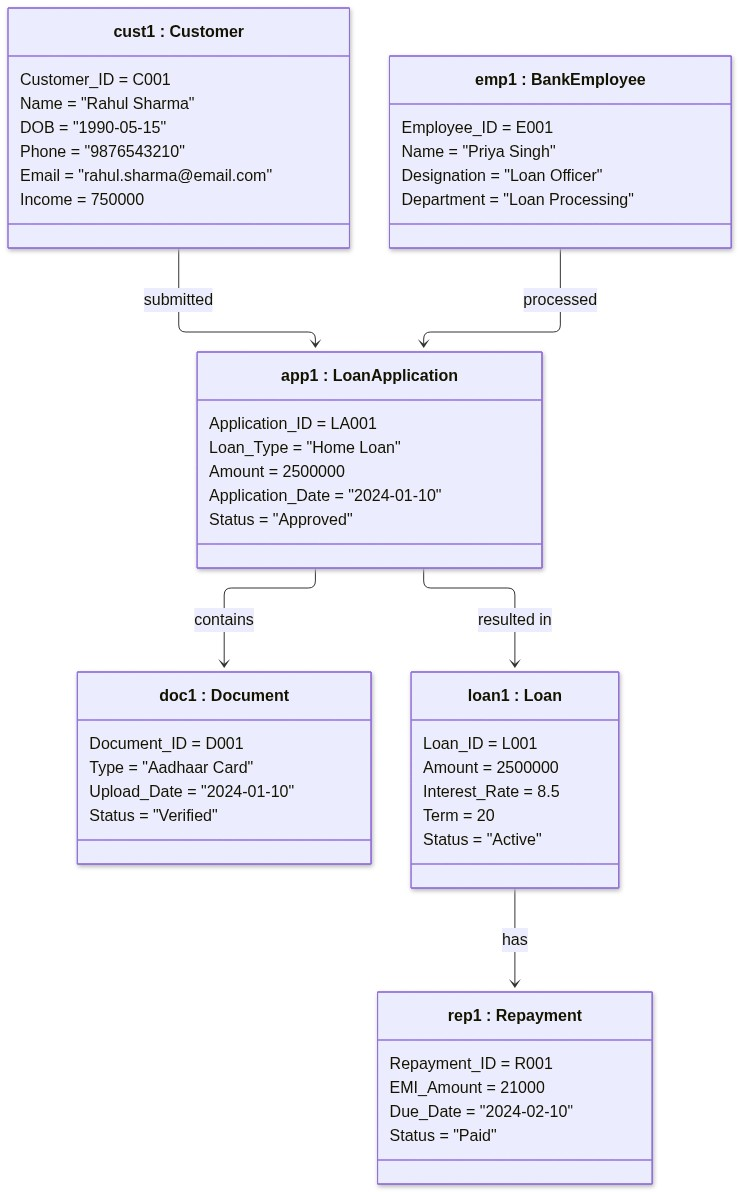
\includegraphics[width=0.85\textwidth]{figures/object_diagram.png}
\caption{Figure 3.9: Object Diagram}
\label{fig:object_diagram}
\end{figure}

\textit{Figure 3.9: Object Diagram}

\section{State-Chart Diagram (Experiment 7)}

The UML State-Chart Diagram captures the dynamic lifecycle of the central domain object: the \textbf{LoanApplication}. It depicts the finite collection of operational states the application occupies, along with the triggering events, guard conditions, and actions that govern state transitions.

\subsection{Lifecycle State Traversal}

\begin{enumerate}
  \item \textbf{Initial State (●):} The customer initiates a new application.
  \item \textbf{Draft State:} The application is being assembled; applicant enters personal and financial metrics.
\end{enumerate}

\begin{itemize}
  \item \textit{Transition Event:} \texttt{submitApplication()}
\end{itemize}

\begin{enumerate}
  \item \textbf{Submitted State:} Application is locked against applicant modifications and queued for processing.
\end{enumerate}

\begin{itemize}
  \item \textit{Transition Event:} \texttt{assignToEmployee()}
\end{itemize}

\begin{enumerate}
  \item \textbf{Under Verification State:} The assigned credit officer examines submitted KYC and financial proof.
\end{enumerate}

\begin{itemize}
  \item \textit{Guard Condition [Documents Invalid]:} Transitions to \textbf{Rejected} (or back to Draft with re-upload request).
  \item \textit{Guard Condition [Documents Valid]:} Transitions to \textbf{Eligibility Assessment}.
\end{itemize}

\begin{enumerate}
  \item \textbf{Eligibility Assessment State:} Algorithmic credit scoring and debt-to-income analysis evaluate borrower capacity.
\end{enumerate}

\begin{itemize}
  \item \textit{Guard Condition [Credit Score < Threshold]:} Transitions to \textbf{Rejected}.
  \item \textit{Guard Condition [Credit Score >= Threshold]:} Transitions to \textbf{Approved}.
\end{itemize}

\begin{enumerate}
  \item \textbf{Approved State:} Loan proposal receives formal credit sanction.
\end{enumerate}

\begin{itemize}
  \item \textit{Transition Event:} \texttt{disburseFunds()}
\end{itemize}

\begin{enumerate}
  \item \textbf{Active Loan State:} Loan funds are disbursed; account transitions into monthly amortization service.
\end{enumerate}

\begin{itemize}
  \item \textit{Transition Event:} \texttt{repaymentsCompleted()}
\end{itemize}

\begin{enumerate}
  \item \textbf{Closed State:} All scheduled principal, interest, and fee liabilities are discharged.
  \item \textbf{Final State (◉):} The application lifecycle successfully terminates.
\end{enumerate}

\begin{figure}[htbp]
\centering
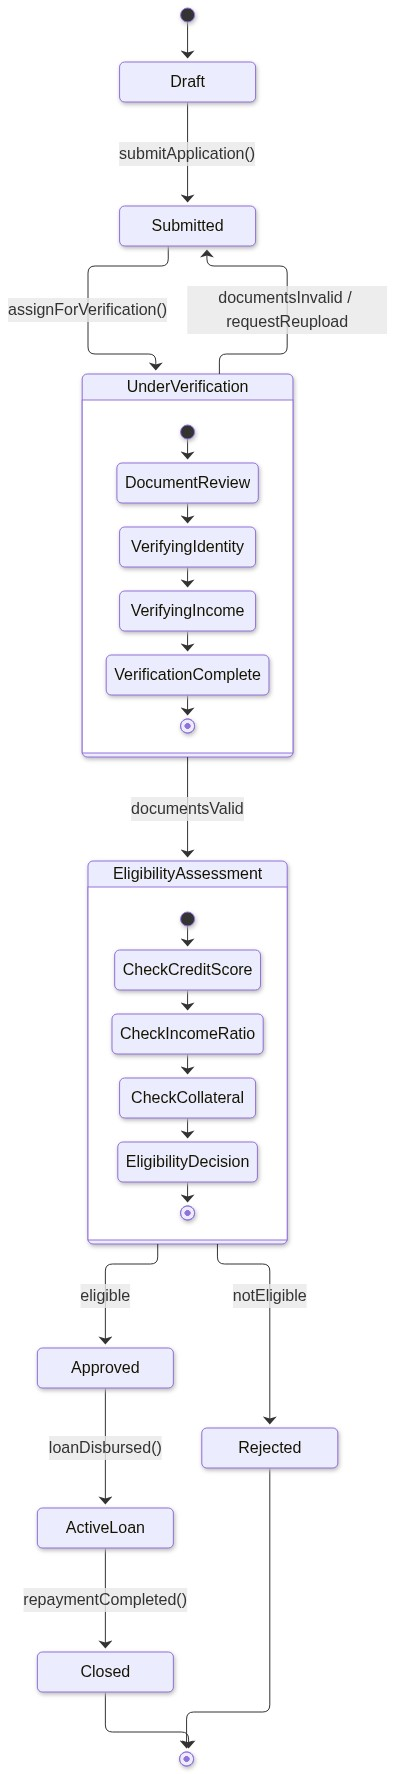
\includegraphics[width=0.85\textwidth]{figures/state_chart.png}
\caption{Figure 3.10: State-Chart Diagram}
\label{fig:state_chart}
\end{figure}

\textit{Figure 3.10: State-Chart Diagram}

\section{Activity Diagram (Experiment 7)}

The UML Activity Diagram represents the procedural business workflow of loan application processing, highlighting concurrency, branch conditions, merge nodes, and organizational responsibilities through swimlanes.

The diagram is organized into three organizational swimlanes:

\begin{enumerate}
  \item \textbf{Customer Swimlane:} Initiates authentication, selects credit products, submits financial metrics, uploads digital attachments, reviews eligibility feedback, and services scheduled repayments.
  \item \textbf{System Swimlane:} Performs automated credential validation, preliminary algorithmic scoring, generates notification emails, computes compound EMI schedules, and updates transaction ledgers.
  \item \textbf{Bank Employee Swimlane:} Inspects uploaded document authenticity, evaluates underwriting risk, validates collateral, and executes formal sanction or rejection authorizations.
\end{enumerate}

The workflow explicitly illustrates decision diamonds governing document validity (\texttt{Are documents valid?}) and credit score thresholds (\texttt{Is customer eligible?}), detailing alternative exception routes to application rejection alongside the critical approval pipeline.

\begin{figure}[htbp]
\centering
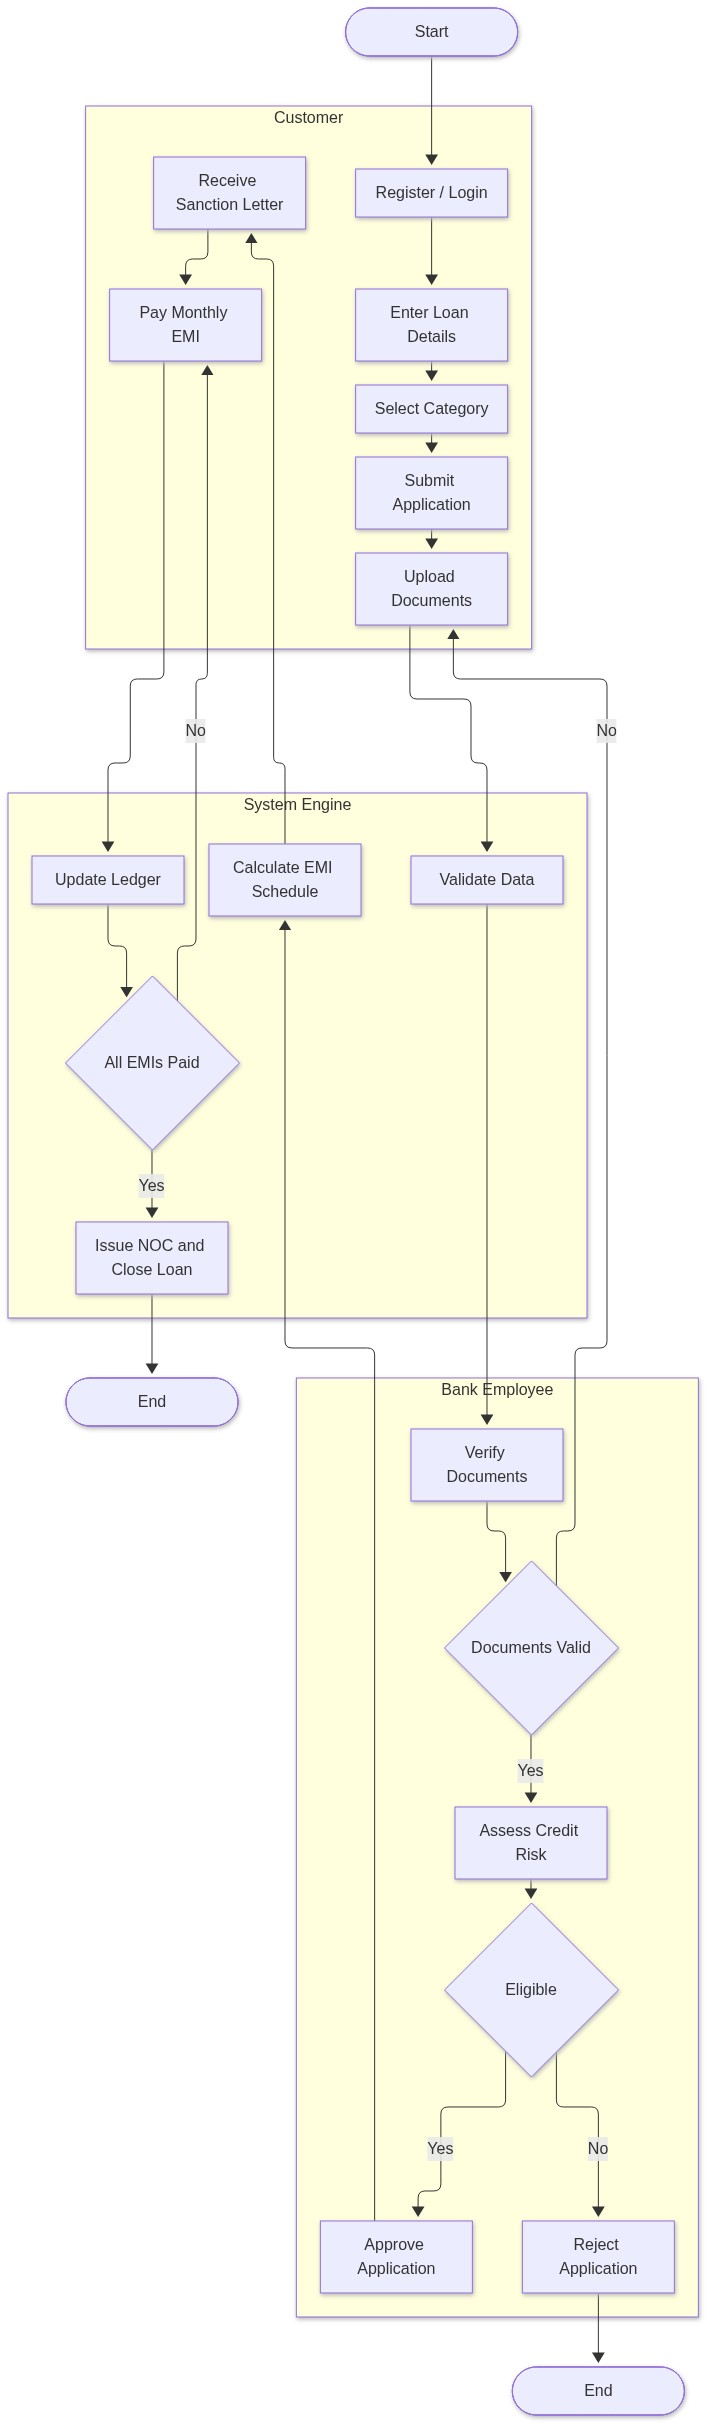
\includegraphics[width=0.85\textwidth]{figures/activity_diagram.png}
\caption{Figure 3.11: Activity Diagram}
\label{fig:activity_diagram}
\end{figure}

\textit{Figure 3.11: Activity Diagram}

\section{Sequence Diagram (Experiment 8)}

The UML Sequence Diagram models the time-ordered exchange of messages between collaborating runtime entities during the primary loan application and approval scenario. The horizontal axis represents participating objects, while the vertical axis represents the chronologically descending progression of time.

\subsection{Participating Lifelines}

\begin{enumerate}
  \item \texttt{c:Customer} (External Actor)
  \item \texttt{ui:LoanApplicationUI} (Boundary/Presentation Layer)
  \item \texttt{ctrl:LoanController} (Control/Business Logic Layer)
  \item \texttt{ver:VerificationEngine} (Domain Service Layer)
  \item \texttt{emp:BankEmployee} (Actor Lifeline)
  \item \texttt{db:LoanDatabase} (Data Access/Persistence Layer)
\end{enumerate}

\subsection{Interaction Sequence}

The sequence commences with customer credentials being validated through \texttt{ctrl:LoanController}. Upon authentication, the customer submits the loan application payload via \texttt{ui:LoanApplicationUI}, which passes execution control to \texttt{ctrl:LoanController}. The controller creates a pending record via \texttt{db:LoanDatabase} and dispatches document validation requests to \texttt{ver:VerificationEngine}. Once automated checks succeed, \texttt{ctrl:LoanController} pushes the application onto the review dashboard of \texttt{emp:BankEmployee}.

An \texttt{alt} combined fragment models the conditional branching of credit underwriting:

\begin{itemize}
  \item \textbf{[Approved Path]:} The employee triggers \texttt{approveApplication()}, prompting \texttt{ctrl:LoanController} to compute the amortization schedule, update the status in \texttt{db:LoanDatabase} to 'Approved', and dispatch a digital sanction notification to \texttt{c:Customer}.
  \item \textbf{[Rejected Path]:} The employee triggers \texttt{rejectApplication(reason)}, updating database state to 'Rejected' and emitting an explanatory rejection notice to \texttt{c:Customer}.
\end{itemize}

\begin{figure}[htbp]
\centering
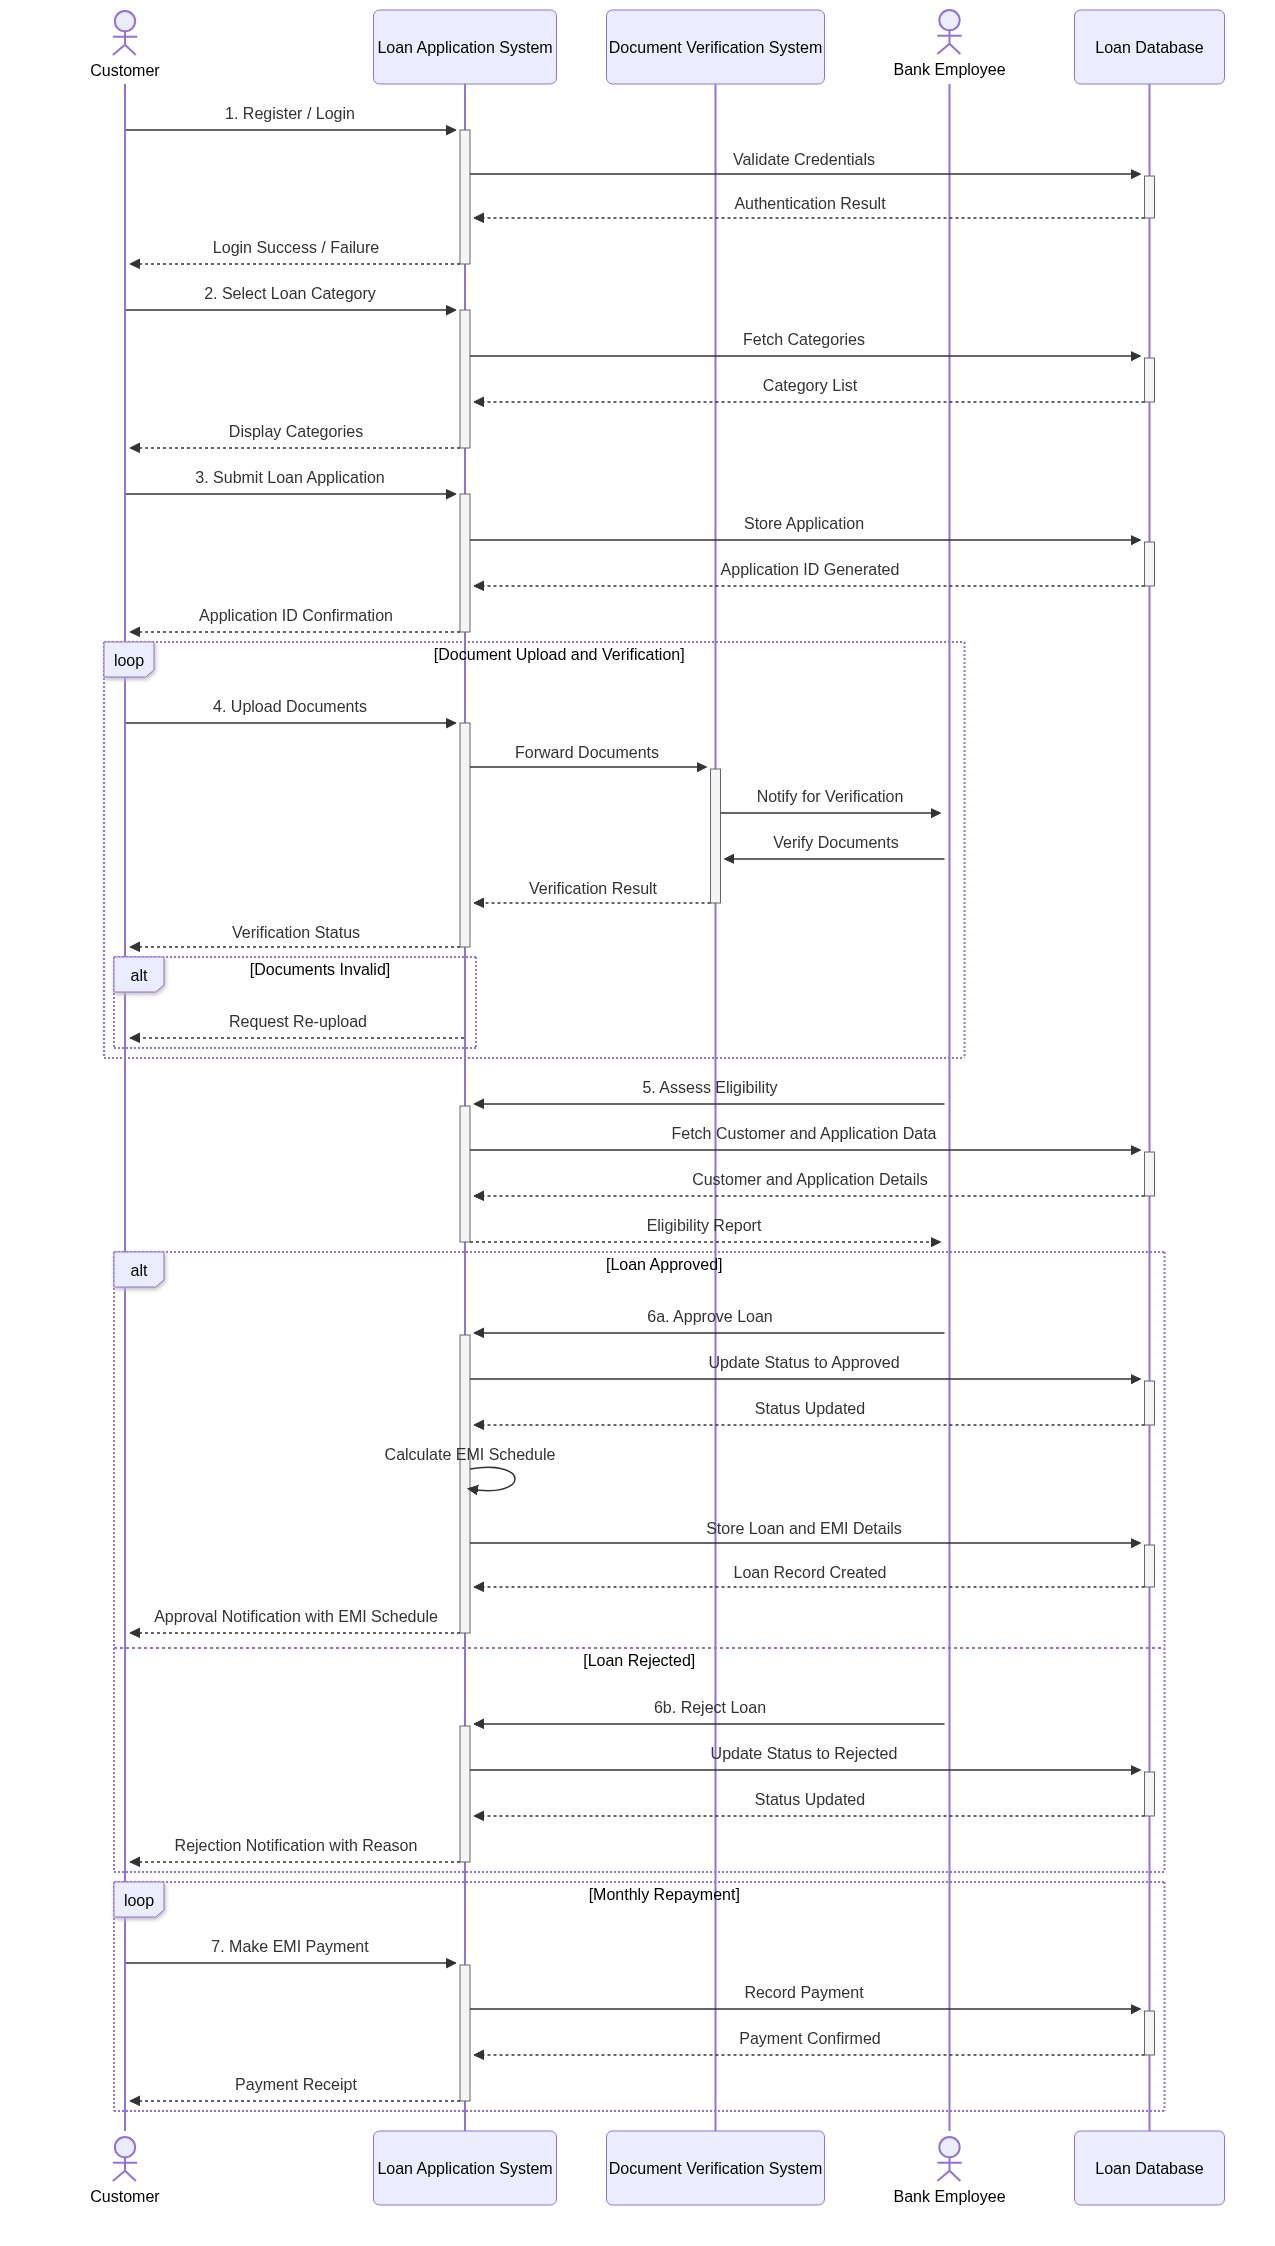
\includegraphics[width=0.85\textwidth]{figures/sequence_diagram.png}
\caption{Figure 3.12: Sequence Diagram}
\label{fig:sequence_diagram}
\end{figure}

\textit{Figure 3.12: Sequence Diagram}

\section{Collaboration Diagram (Communication Diagram) (Experiment 8)}

The UML Collaboration (Communication) Diagram models the structural relationships and communication pathways between participating objects, emphasizing the architecture of object links while preserving chronological sequencing through hierarchical message numbering.

Representing the identical scenario detailed in the Sequence Diagram, the Collaboration Diagram utilizes numbered message links to trace the flow of control:

\begin{enumerate}
  \item \texttt{1: authenticate(credentials)} - Customer to LoanApplicationUI
  \item \texttt{2: submitApplication(loanData)} - Customer to LoanApplicationUI
  \item \texttt{3: persistApplication(loanData)} - LoanApplicationUI to LoanController
  \item \texttt{4: insertRecord(loanData)} - LoanController to LoanDatabase
  \item \texttt{5: uploadDocuments(docFiles)} - Customer to LoanApplicationUI
  \item \texttt{6: verifyDocuments(docFiles)} - LoanController to VerificationEngine
  \item \texttt{7: assignToReviewQueue(appId)} - LoanController to BankEmployee
  \item \texttt{8: submitDecision(appId, decision)} - BankEmployee to LoanController
  \item \texttt{9: updateStatus(appId, decision)} - LoanController to LoanDatabase
  \item \texttt{10: notifyCustomer(decision)} - LoanController to Customer
\end{enumerate}

\begin{figure}[htbp]
\centering
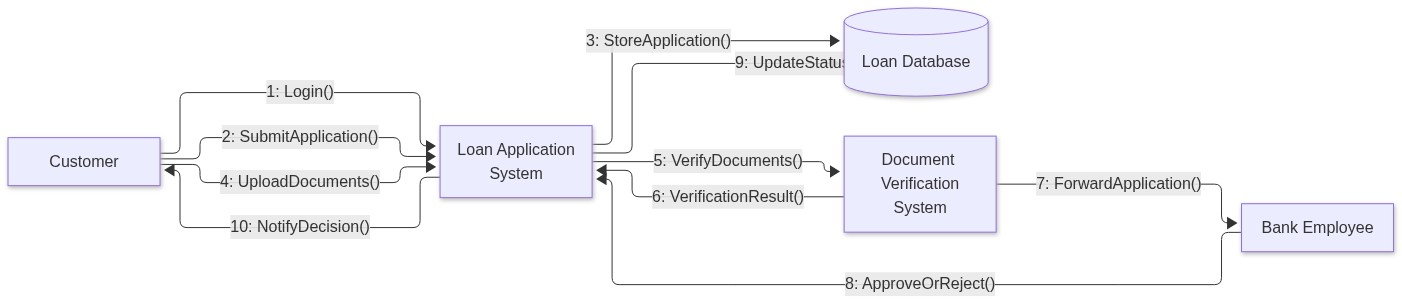
\includegraphics[width=0.85\textwidth]{figures/collaboration_diagram.png}
\caption{Figure 3.13: Collaboration Diagram}
\label{fig:collaboration_diagram}
\end{figure}

\textit{Figure 3.13: Collaboration Diagram}

\section{Component Diagram}

The UML Component Diagram documents the high-level software architecture, depicting the physical software modules (components), their provided/required interfaces, and runtime dependencies.

The Bank Loan Management System is architectured according to a robust three-tier modular pattern:

\begin{enumerate}
  \item \textbf{Presentation Tier:} Comprises the \texttt{Web Browser UI} component and \texttt{Client-Side Routing / Form Validation} modules delivering responsive HTML5/CSS3/JavaScript interfaces.
  \item \textbf{Business Logic Tier:} Implements decoupled enterprise components:
\end{enumerate}

\begin{itemize}
  \item \texttt{Authentication Module}: Enforces JWT-based role authorization and session control.
  \item \texttt{Loan Application Module}: Manages application ingestion and lifecycle state.
  \item \texttt{Document Management Module}: Handles file upload encryption and storage indexing.
  \item \texttt{Underwriting \& Verification Module}: Executes automated eligibility scoring rules.
  \item \texttt{EMI \& Repayment Engine}: Computes mathematical amortization tables.
  \item \texttt{Reporting \& Analytics Service}: Compiles cross-functional BI metrics.
  \item \texttt{Notification Service}: Interacts with asynchronous email/SMS gateways.
\end{itemize}

\begin{enumerate}
  \item \textbf{Data Access Tier:} Encapsulates the \texttt{Database Access Object (DAO) Layer} and \texttt{Object-Relational Mapping (ORM)} component mediating data transactions with persistent storage.
\end{enumerate}

\begin{figure}[htbp]
\centering
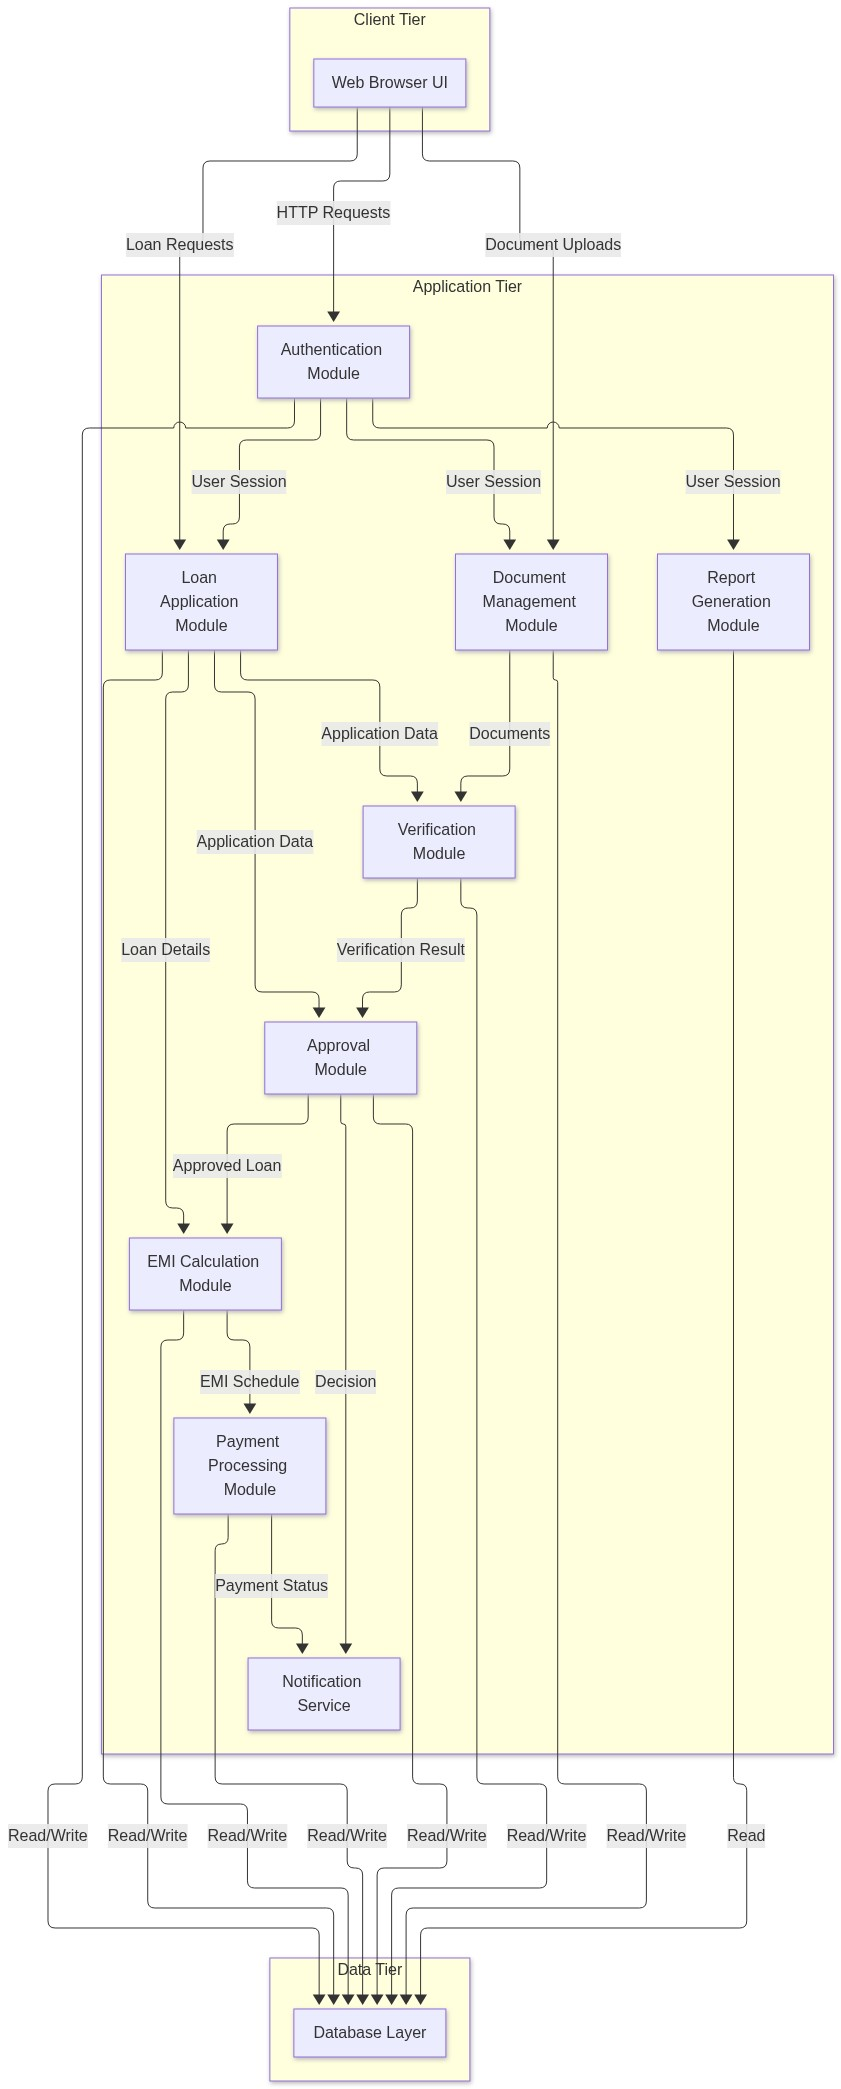
\includegraphics[width=0.85\textwidth]{figures/component_diagram.png}
\caption{Figure 3.14: Component Diagram}
\label{fig:component_diagram}
\end{figure}

\textit{Figure 3.14: Component Diagram}

\section{Deployment Diagram}

The UML Deployment Diagram illustrates the physical runtime environment, showing the hardware nodes, execution environments, network topologies, and communication protocols that host the software system.

The enterprise deployment topology consists of four distinct architectural tiers:

\begin{enumerate}
  \item \textbf{Client Tier:} Standard workstations and mobile devices executing modern web browsers (Chrome, Edge, Firefox), communicating over encrypted HTTPS (TLS 1.3) via Port 443.
  \item \textbf{Web / Application Server (DMZ):} A high-performance enterprise application server (e.g., Apache/Nginx reverse proxy fronting Python/Java application servers) hosting containerized business services, session caches, and API routers.
  \item \textbf{Database Server (Secure Internal Network):} A dedicated, secured database cluster executing MySQL/PostgreSQL with automated replication and continuous WAL archiving, communicating over TCP/IP via Port 3306 behind an internal firewall.
  \item \textbf{Document Storage Server:} A secure storage repository (dedicated NAS / encrypted object store) safeguarding sensitive customer KYC attachments and signed loan contracts.
  \item \textbf{External Services:} Interconnected via secure REST APIs over HTTPS to external credit score bureaus and SMTP notification servers.
\end{enumerate}

\begin{figure}[htbp]
\centering
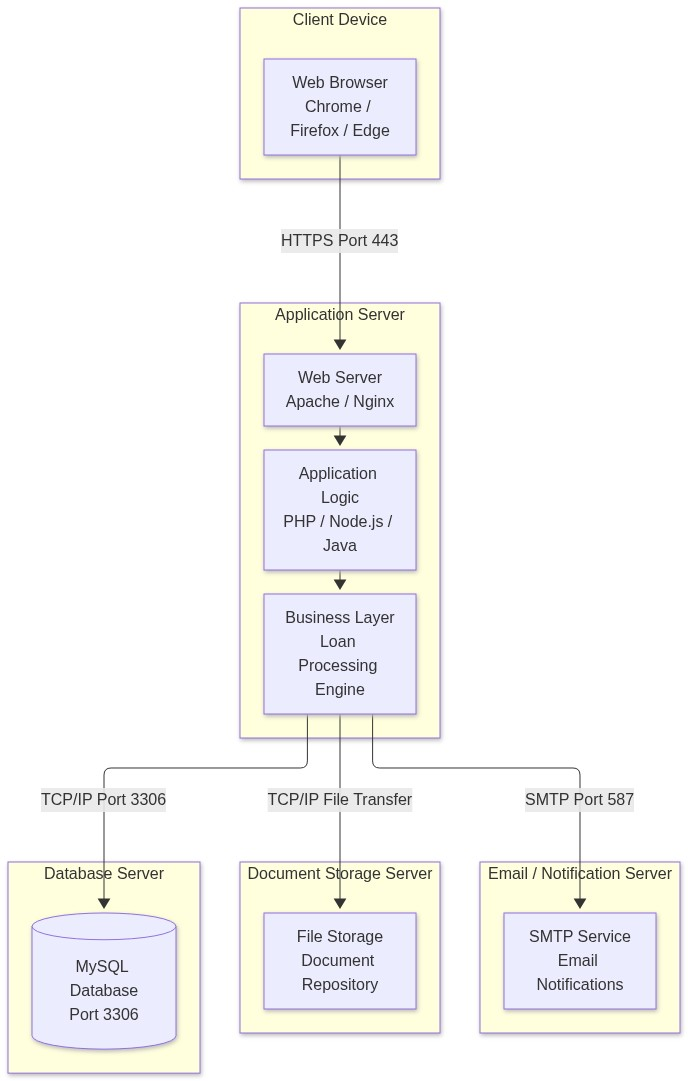
\includegraphics[width=0.85\textwidth]{figures/deployment_diagram.png}
\caption{Figure 3.15: Deployment Diagram}
\label{fig:deployment_diagram}
\end{figure}

\textit{Figure 3.15: Deployment Diagram}
